% Options for packages loaded elsewhere
\PassOptionsToPackage{unicode}{hyperref}
\PassOptionsToPackage{hyphens}{url}
%
\documentclass[
]{article}
\usepackage{amsmath,amssymb}
\usepackage{lmodern}
\usepackage{iftex}
\ifPDFTeX
  \usepackage[T1]{fontenc}
  \usepackage[utf8]{inputenc}
  \usepackage{textcomp} % provide euro and other symbols
\else % if luatex or xetex
  \usepackage{unicode-math}
  \defaultfontfeatures{Scale=MatchLowercase}
  \defaultfontfeatures[\rmfamily]{Ligatures=TeX,Scale=1}
\fi
% Use upquote if available, for straight quotes in verbatim environments
\IfFileExists{upquote.sty}{\usepackage{upquote}}{}
\IfFileExists{microtype.sty}{% use microtype if available
  \usepackage[]{microtype}
  \UseMicrotypeSet[protrusion]{basicmath} % disable protrusion for tt fonts
}{}
\makeatletter
\@ifundefined{KOMAClassName}{% if non-KOMA class
  \IfFileExists{parskip.sty}{%
    \usepackage{parskip}
  }{% else
    \setlength{\parindent}{0pt}
    \setlength{\parskip}{6pt plus 2pt minus 1pt}}
}{% if KOMA class
  \KOMAoptions{parskip=half}}
\makeatother
\usepackage{xcolor}
\IfFileExists{xurl.sty}{\usepackage{xurl}}{} % add URL line breaks if available
\IfFileExists{bookmark.sty}{\usepackage{bookmark}}{\usepackage{hyperref}}
\hypersetup{
  hidelinks,
  pdfcreator={LaTeX via pandoc}}
\urlstyle{same} % disable monospaced font for URLs
\usepackage{longtable,booktabs,array}
\usepackage{calc} % for calculating minipage widths
% Correct order of tables after \paragraph or \subparagraph
\usepackage{etoolbox}
\makeatletter
\patchcmd\longtable{\par}{\if@noskipsec\mbox{}\fi\par}{}{}
\makeatother
% Allow footnotes in longtable head/foot
\IfFileExists{footnotehyper.sty}{\usepackage{footnotehyper}}{\usepackage{footnote}}
\makesavenoteenv{longtable}
\usepackage{graphicx}
\makeatletter
\def\maxwidth{\ifdim\Gin@nat@width>\linewidth\linewidth\else\Gin@nat@width\fi}
\def\maxheight{\ifdim\Gin@nat@height>\textheight\textheight\else\Gin@nat@height\fi}
\makeatother
% Scale images if necessary, so that they will not overflow the page
% margins by default, and it is still possible to overwrite the defaults
% using explicit options in \includegraphics[width, height, ...]{}
\setkeys{Gin}{width=\maxwidth,height=\maxheight,keepaspectratio}
% Set default figure placement to htbp
\makeatletter
\def\fps@figure{htbp}
\makeatother
\setlength{\emergencystretch}{3em} % prevent overfull lines
\providecommand{\tightlist}{%
  \setlength{\itemsep}{0pt}\setlength{\parskip}{0pt}}
\setcounter{secnumdepth}{-\maxdimen} % remove section numbering
\ifLuaTeX
  \usepackage{selnolig}  % disable illegal ligatures
\fi

\author{}
\date{}

\begin{document}

\tableofcontents

\hypertarget{ux9ad8ux4e2dux57faux7840ux7bc7}{%
\section{高中基础篇}\label{ux9ad8ux4e2dux57faux7840ux7bc7}}

\begin{quote}
本部分主要是对现行高中课本的补充,\\
大多是过于抽象的概念,看看就行了。
\end{quote}

\hypertarget{ux7b2cux4e00ux7ae0--ux5e42ux51fdux6570ux6307ux6570ux51fdux6570ux548cux5bf9ux6570ux51fdux6570}{%
\subsubsection{第一章
幂函数、指数函数和对数函数}\label{ux7b2cux4e00ux7ae0--ux5e42ux51fdux6570ux6307ux6570ux51fdux6570ux548cux5bf9ux6570ux51fdux6570}}

\hypertarget{ux4e00--ux96c6ux5408}{%
\paragraph{一 集合}\label{ux4e00--ux96c6ux5408}}

\hypertarget{11--ux96c6ux5408}{%
\subparagraph{1.1 集合}\label{11--ux96c6ux5408}}

\textbf{集合}(简称\textbf{集}):一组对象的全体.\\
\textbf{元素}: 集合里的各个对象.\\
\textbf{有限集}:含有有限个元素的集合.\\
\textbf{无限集}:含有无限个元素的集合.\\
集合的性质:

\begin{itemize}
\item
  \textbf{确定性}
\item
  \textbf{互异性}
\item
  \textbf{无序性}
\end{itemize}

集合的表示方法:

\begin{itemize}
\item
  \textbf{列举法}: \\
  把元素中的元素一一列举出来,写在大括号内表示集合的方法.
\item
  \textbf{描述法}:\\
  把集合中的元素公共属性描述出来,写在大括号内表示集合的方法.\\
  集合同元素的关系:
\item
  \textbf{属于}(\textbf{\(\in\)})
\item
  \textbf{不属于}(\textbf{\(\notin\)})
\end{itemize}

\hypertarget{ux4e8c--ux6620ux5c04ux4e0eux51fdux6570}{%
\paragraph{二 映射与函数}\label{ux4e8c--ux6620ux5c04ux4e0eux51fdux6570}}

\hypertarget{ux4e09--ux5e42ux51fdux6570}{%
\paragraph{三 幂函数}\label{ux4e09--ux5e42ux51fdux6570}}

\hypertarget{ux56db--ux6307ux6570ux51fdux6570ux548cux5bf9ux6570ux51fdux6570}{%
\paragraph{四
指数函数和对数函数}\label{ux56db--ux6307ux6570ux51fdux6570ux548cux5bf9ux6570ux51fdux6570}}

\hypertarget{ux7b2cux4e8cux7ae0--ux4e09ux89d2ux51fdux6570}{%
\subsubsection{第二章
三角函数}\label{ux7b2cux4e8cux7ae0--ux4e09ux89d2ux51fdux6570}}

\hypertarget{ux4e00--ux4efbux610fux89d2ux7684ux4e09ux89d2ux51fdux6570}{%
\paragraph{一
任意角的三角函数}\label{ux4e00--ux4efbux610fux89d2ux7684ux4e09ux89d2ux51fdux6570}}

\hypertarget{21--ux89d2ux7684ux6982ux5ff5ux7684ux63a8ux5e7f}{%
\subparagraph{2.1
角的概念的推广}\label{21--ux89d2ux7684ux6982ux5ff5ux7684ux63a8ux5e7f}}

\textbf{角}: 由一条射线绕着它的端点旋转而成.

\begin{itemize}
\item
  \textbf{始边}: 旋转开始时的射线.
\item
  \textbf{终边}: 旋转终止时的射线.
\item
  \textbf{顶点}: 射线的端点.
\end{itemize}

角的分类:

\begin{itemize}
\item
  \textbf{正角}: 按逆时针方向旋转所形成的角.
\item
  \textbf{负角}: 按顺时针方向旋转所形成的角.
\item
  \textbf{零角}: 未做任何旋转所形成的角.
\item
  \textbf{象限角}: 角的终边在第几象限,就说这个角是第几象限的角
  (或说这个角属于第几象限) .
\item
  \textbf{轴线角}: 角的终边在坐标轴上.
\end{itemize}

一般地,\textbf{所有与\(\alpha\)角终边相同的角,连同\(\alpha\)角在内
(而且只有这样的角) ,可以用式子\\
\(2k\pi + \alpha, k \in \mathbb Z\)\\
来表示.组成的集合可记作:\\
\( \{\beta | \beta = 2k\pi + \alpha, k \in \mathbb Z \} \)}

\hypertarget{22--ux5f27ux5ea6ux5236}{%
\subparagraph{2.2 弧度制}\label{22--ux5f27ux5ea6ux5236}}

\textbf{角度}:

\begin{itemize}
\item
  周角的\(\frac{1}{360}\)为\(1^{\circ}\)的角.
\end{itemize}

\textbf{角度制}:

\begin{itemize}
\item
  用角度做单位来度量角的制度.
\end{itemize}

\textbf{弧度}:

\begin{itemize}
\item
  等于半径长的圆弧所对的圆心角为\(1 \mathrm{rad}\)的角.
\end{itemize}

\textbf{弧度制}:

\begin{itemize}
\item
  用弧度做单位来度量角的制度.
\end{itemize}

一般地,\textbf{正角的弧度数为正数,负角的弧度数为负数,零角的弧度数为零,任一已知角\(\alpha\)的弧度数的绝对值\(\left| \alpha \right|=  \frac{l}{r}\),其中\(l\)为以\(\alpha\)作为圆心角时所对圆弧的长\(r\)为圆的半径.}

\textbf{圆弧长公式}:\(l =\left| \alpha \right| r\)\\
\textbf{扇形面积公式}:\(S = {l \over R} \cdot {1 \over 2\pi} \cdot \pi R^2 = {1 \over 2}\left| \alpha \right| R^2 ={1 \over 2}lR\)\\

\hypertarget{23--ux4efbux610fux89d2ux7684ux4e09ux89d2ux51fdux6570}{%
\subparagraph{2.3
任意角的三角函数}\label{23--ux4efbux610fux89d2ux7684ux4e09ux89d2ux51fdux6570}}

设\(\alpha\)是一个任意大小的角.角\(\alpha\)的终边上任意一点\(P\)的坐标是\((x,y)\),它与原点的距离是\(r(r >0)\),那么角\(\alpha\)的\textbf{正弦}、\textbf{余弦}、\textbf{正切}、\textbf{余切}、\textbf{正割}、\textbf{余割}分别是

\begin{longtable}[]{@{}lllllll@{}}
\toprule
三角函数 & 定义 & 定义域\((k \in \mathbb Z)\) & Ⅰ & Ⅱ & Ⅲ & Ⅳ \\
\midrule
\endhead
正弦函数\(\sin(\alpha)\) & \(\frac{y}{r}\) & \(\alpha \in \mathbb R\) &
+ & + & - & - \\
余弦函数\(\cos(\alpha)\) & \(\frac{x}{r}\) & \(\alpha \in \mathbb R\) &
+ & - & - & + \\
正切函数\(\tan(\alpha)\) & \(\frac{y}{x}\) & \(\alpha \in \mathbb R\) 且
\(\alpha \neq {\pi \over 2} + k\pi\) & + & - & + & - \\
余切函数\(\cot(\alpha)\) & \(\frac{x}{y}\) & \(\alpha \in \mathbb R\) 且
\(\alpha \neq k\pi\) & + & - & + & - \\
正割函数\(\sec(\alpha)\) & \(\frac{r}{x}\) & \(\alpha \in \mathbb R\) 且
\(\alpha \neq {\pi \over 2} + k\pi \) & + & - & - & + \\
余割函数\(\csc(\alpha)\) & \(\frac{r}{y}\) & \(\alpha \in \mathbb R\) 且
\(\alpha \neq k\pi\) & + & + & - & - \\
\bottomrule
\end{longtable}

\hypertarget{24--ux540cux89d2ux4e09ux89d2ux51fdux6570ux7684ux57faux672cux5173ux7cfbux5f0f}{%
\subparagraph{2.4
同角三角函数的基本关系式}\label{24--ux540cux89d2ux4e09ux89d2ux51fdux6570ux7684ux57faux672cux5173ux7cfbux5f0f}}

\begin{enumerate}
\def\labelenumi{\arabic{enumi}.}
\item
  倒数关系:
\end{enumerate}

\begin{itemize}
\item
  \(\sin(\alpha)\csc(\alpha) = 1\)
\item
  \(\cos(\alpha)\sec(\alpha) = 1\)
\item
  \(\tan(\alpha)\cot(\alpha) = 1\)
\end{itemize}

\begin{enumerate}
\def\labelenumi{\arabic{enumi}.}
\item
  商数关系:
\end{enumerate}

\begin{itemize}
\item
  \(\tan(\alpha) = {\sin(\alpha) \over \cos(\alpha)}\)
\item
  \(\cot(\alpha) = {\cos(\alpha) \over \sin(\alpha)}\)
\end{itemize}

\begin{enumerate}
\def\labelenumi{\arabic{enumi}.}
\item
  平方关系:
\end{enumerate}

\begin{itemize}
\item
  \(\sin^2(\alpha) + \cos^2(\alpha) = 1\)
\item
  \(\tan^2(\alpha) + 1 = \sec^2(\alpha)\)
\item
  \(\cot^2(\alpha) + 1 = \csc^2(\alpha)\)
\end{itemize}

上述各式均为\textbf{恒等式}.

\hypertarget{25--ux8bf1ux5bfcux516cux5f0f}{%
\subparagraph{2.5 诱导公式}\label{25--ux8bf1ux5bfcux516cux5f0f}}

\(\sec(\alpha)\)与\(\csc(\alpha)\)并不常用,故下表省略.

\begin{longtable}[]{@{}llllll@{}}
\toprule
& \(-\alpha\) & \(\pi - \alpha\) & \(\pi + \alpha\) & \(2\pi - \alpha\)
& \(2k\pi + \alpha\) \\
\midrule
\endhead
\(\sin\) & - & + & - & - & + \\
\(\cos\) & + & - & - & + & + \\
\(\tan\) & - & - & + & - & + \\
\(\cot\) & - & - & + & - & + \\
\bottomrule
\end{longtable}

概括:\textbf{\(-\alpha\),\(\pi - \alpha\),\(\pi + \alpha\),\(2\pi - \alpha\),\(2k\pi + \alpha\)的三角函数值等于\(\alpha\)的同名函数值,前面加上一个把\(\alpha\)看成锐角时原函数值的符号.}

\hypertarget{ux4e8c--ux4e09ux89d2ux51fdux6570ux7684ux56feux50cfux548cux6027ux8d28}{%
\paragraph{二
三角函数的图像和性质}\label{ux4e8c--ux4e09ux89d2ux51fdux6570ux7684ux56feux50cfux548cux6027ux8d28}}

\textbf{性质}:

\begin{longtable}[]{@{}llllll@{}}
\toprule
函数名 & 奇偶性 & 周期性 & 有界性 & 一阶导数 & 二阶导数 \\
\midrule
\endhead
\(\sin(x)\) & 奇 & \(T = 2\pi\) & 1 & \(\cos(x)\) & \(-\sin(x)\) \\
\(\cos(x)\) & 偶 & \(T = 2\pi\) & 1 & \(-\sin(x)\) & \(-\cos(x)\) \\
\(\tan(x)\) & 奇 & \(T = \pi\) & 无界 &
\({\sin^2(x) + \cos^2(x)}\over \cos^2(x)\) &
\({2\sin(x)\cos^2(x) + \sin^3(x)}\over \cos^3(x)\) \\
\(\cot(x)\) & 奇 & \(T = \pi\) & 无界 & \(-{1 \over \sin^2(x)}\) &
\({2\sin^2(x)\cos(x)+2\cos^3(x)}\over \sin^3(x)\) \\
\(\sec(x)\) & 奇 & \(T = 2\pi\) & 无界 & \(\sin(x) \over \cos^2(x)\) &
\({\cos^2(x) + 2\sin^2(x)}\over \cos^3(x)\) \\
\(\csc(x)\) & 偶 & \(T = 2\pi\) & 无界 & \(-{\cos(x) \over \sin^2(x)}\)
& \(-{{2\cos(x) + \sin^2(x)}\over \sin^3(x)}\) \\
\bottomrule
\end{longtable}

\textbf{图像}(一个最小正周期内):由上表,可得\\
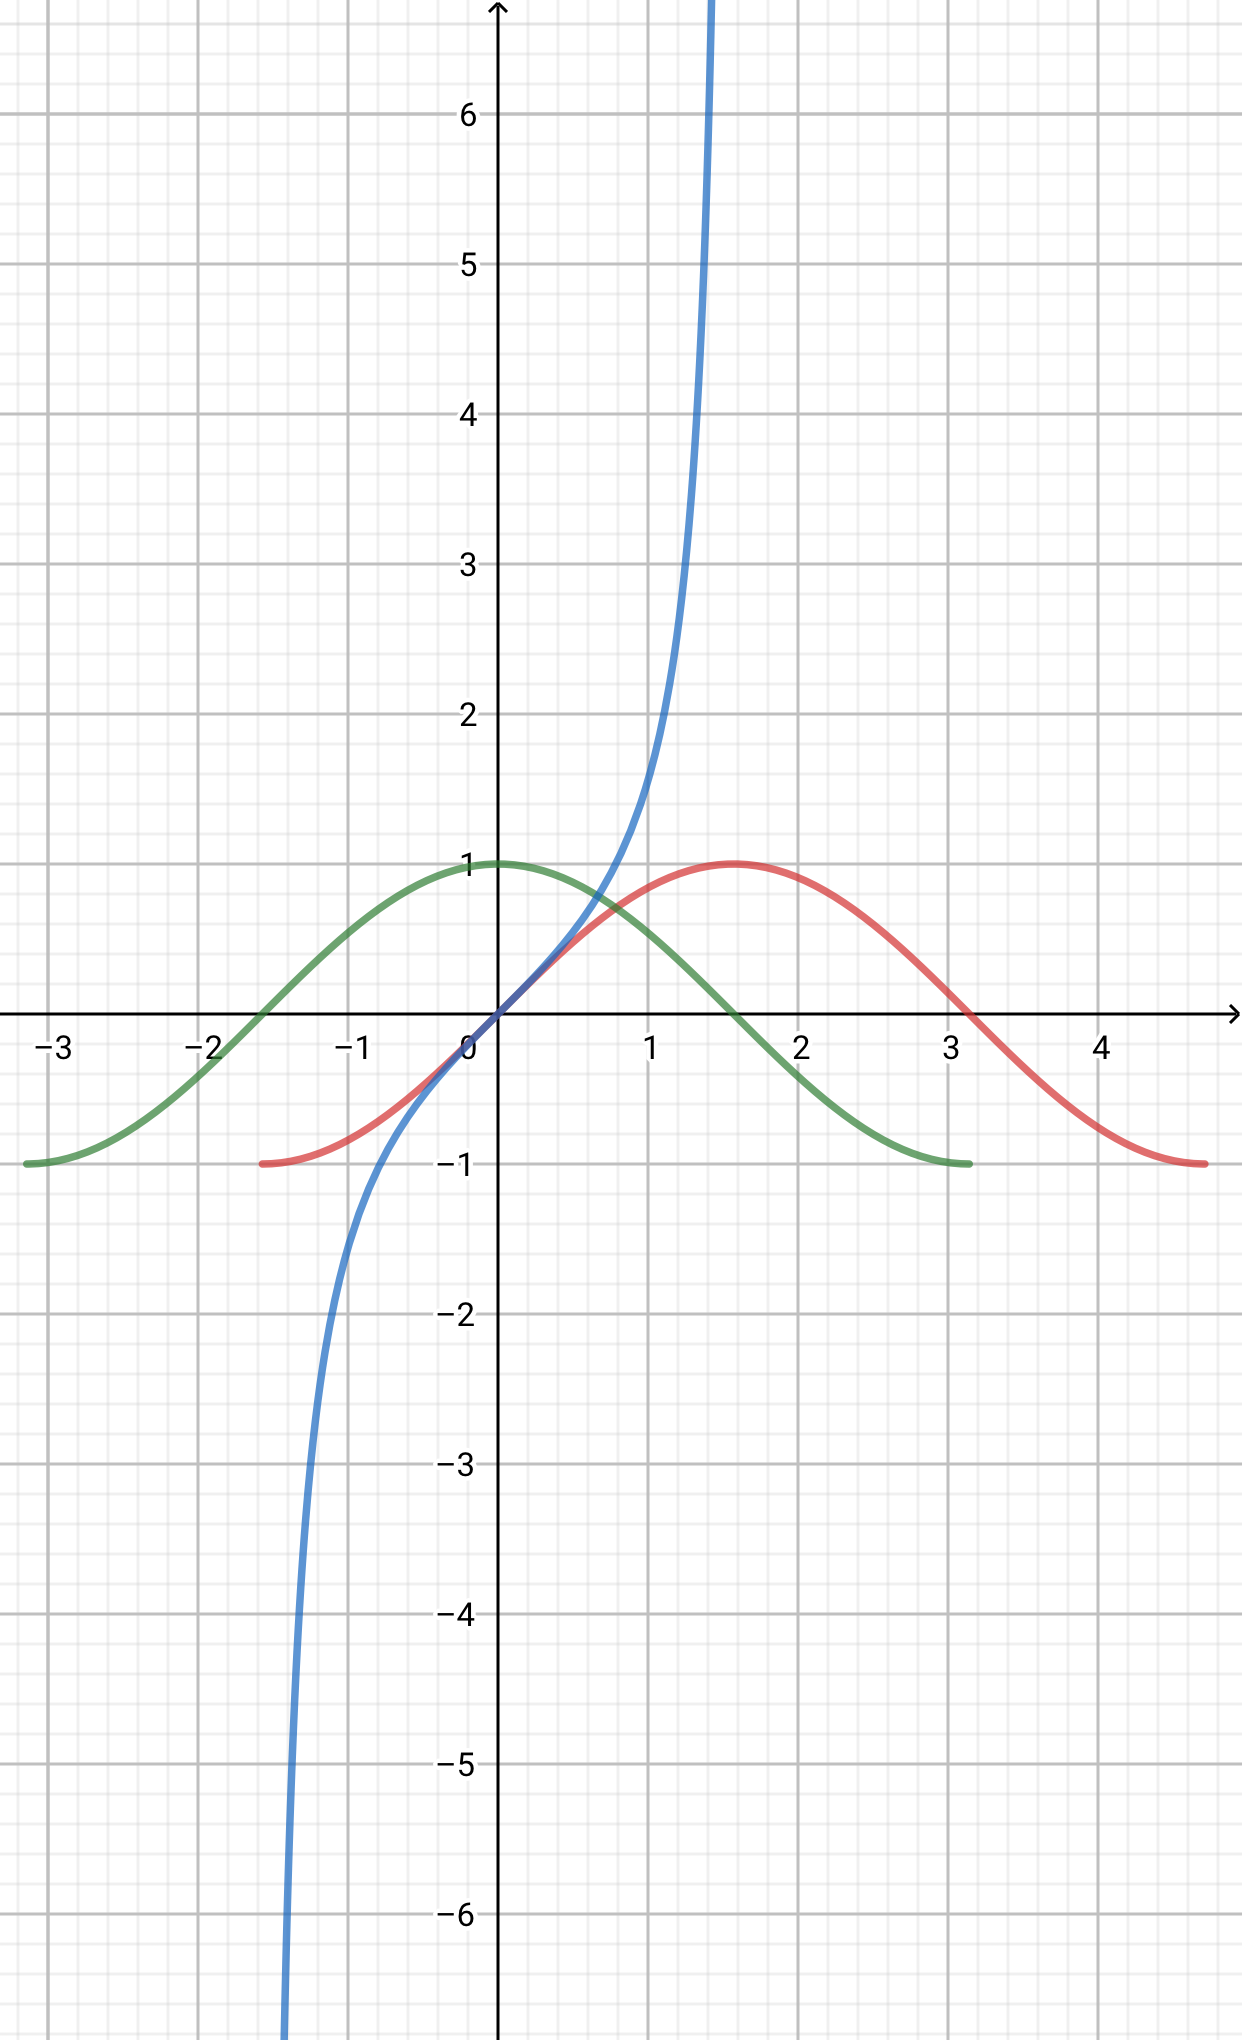
\includegraphics{C:/Users/Administrator/iCloudDrive/iCloud~com~coderforart~iOS~MWeb/The-collections-of-notes-and-mistakes/note/Mathematics/media/16495610024847.png}

\hypertarget{ux51fdux6570y--asinomega-x--varphi-a--0-omega--0-0-leqslant-varphi--2pi-x-in-mathbb-rux7684ux56feux50cf}{%
\subparagraph{\texorpdfstring{函数\(y = A\sin(\omega x + \varphi), (A > 0, \omega > 0, 0 \leqslant \varphi < 2\pi), x \in \mathbb R\)的图像}{函数y = A\textbackslash sin(\textbackslash omega x + \textbackslash varphi), (A \textgreater{} 0, \textbackslash omega \textgreater{} 0, 0 \textbackslash leqslant \textbackslash varphi \textless{} 2\textbackslash pi), x \textbackslash in \textbackslash mathbb R的图像}}\label{ux51fdux6570y--asinomega-x--varphi-a--0-omega--0-0-leqslant-varphi--2pi-x-in-mathbb-rux7684ux56feux50cf}}

\textbf{作法}:

\begin{enumerate}
\def\labelenumi{\arabic{enumi}.}
\item
  作出\(y = \sin(x)\)
\item
  向左平移\(\varphi\)个单位
\item
  横坐标缩短到原来的\(1 \over \omega\)倍
\item
  纵坐标伸长到原来的\(A\)倍
\end{enumerate}

表示振动量时参数含义:

\begin{itemize}
\item
  \textbf{振幅}\(A\)
\item
  \textbf{周期}\(T = {2\pi \over \omega}\)
\item
  \textbf{频率}\(f = {1 \over T} = {\omega \over 2\pi}\)
\item
  \textbf{相位}\(\omega x + \varphi\)
\item
  \textbf{初相}\(\varphi\)
\end{itemize}

\hypertarget{ux7b2cux4e09ux7ae0-ux4e24ux89d2ux548cux4e0eux5deeux7684ux4e09ux89d2ux51fdux6570ux516cux5f0f}{%
\subsubsection{第三章
两角和与差的三角函数公式}\label{ux7b2cux4e09ux7ae0-ux4e24ux89d2ux548cux4e0eux5deeux7684ux4e09ux89d2ux51fdux6570ux516cux5f0f}}

\hypertarget{ux4e24ux89d2ux548cux4e0eux5dee}{%
\paragraph{两角和与差}\label{ux4e24ux89d2ux548cux4e0eux5dee}}

\begin{itemize}
\item
  \(C_{\alpha \pm \beta}\):\\
  \(\cos(\alpha \pm \beta) = \cos(\alpha)\cos(\beta) \mp \sin(\alpha)\sin(\beta)\)
\item
  \(S_{\alpha \pm \beta}\):\\
  \(\sin(\alpha \pm \beta) = \sin(\alpha)\cos(\beta) \pm \sin(\beta)\cos(\alpha)\)
\item
  \(T_{\alpha \pm \beta}\):\\
  \(\tan(\alpha \pm \beta) = {{\tan(\alpha) \pm \tan(\beta)} \over {1 \mp \tan(\alpha)\tan(\beta)}}\)
\end{itemize}

\hypertarget{ux500dux89d2}{%
\paragraph{倍角}\label{ux500dux89d2}}

\begin{enumerate}
\def\labelenumi{\arabic{enumi}.}
\item
  二倍角
\end{enumerate}

\begin{itemize}
\item
  \(S_{2\alpha}\):\\
  \(\sin(2\alpha) = 2\sin(\alpha)\cos(\alpha)\)
\item
  \(C_{2\alpha}\):\\
  \(\cos(2\alpha) = \cos^2(\alpha) - \sin^2(\alpha)\)
\item
  \(C_{2\alpha}^\prime\):

  \begin{itemize}
  \item
    \(\cos(2\alpha) = 2\cos^2(\alpha) - 1\)
  \item
    \(\cos(2\alpha) = 1 - 2\sin^2(\alpha)\)
  \end{itemize}
\item
  \(T_{2\alpha}\):\\
  \(\tan(2\alpha) = {2\tan(\alpha) \over {1 - \tan^2\alpha}}\)
\end{itemize}

\begin{enumerate}
\def\labelenumi{\arabic{enumi}.}
\item
  \(n\)倍角
\end{enumerate}

\begin{itemize}
\item
  \(S_{n\alpha}\):\\
  \(\sin(n\alpha) = \begin{vmatrix} \sin(\alpha) & 0 & 0 & \cdots & 0 & 0 \\ 0 & 2\cos(\alpha) & 1 & \cdots & 0 & 0 \\ 0 & 1 & 2\cos(\alpha) & \cdots & 0 & 0 \\ \vdots & \vdots & \vdots & \ddots & 1 & 0 \\ 0 & 0 & 0 & 1 & 2\cos(\alpha) & 1 \\ 0 & 0 & 0 & 0 & 1 & 2\cos(\alpha) \end{vmatrix}\)
\item
  \(C_{n\alpha}\):\\
  \(\cos(n\alpha) = \begin{vmatrix} \cos(\alpha) & 1 & 0 & \cdots & 0 & 0 \\ 1 & 2\cos(\alpha) & 1 & \cdots & 0 & 0 \\ 0 & 1 & 2\cos(\alpha) & \cdots & 0 & 0 \\ \vdots & \vdots & \vdots & \ddots & 1 & 0 \\ 0 & 0 & 0 & 1 & 2\cos(\alpha) & 1 \\ 0 & 0 & 0 & 0 & 1 & 2\cos(\alpha) \end{vmatrix}\)
\end{itemize}

\hypertarget{ux534aux89d2}{%
\paragraph{半角}\label{ux534aux89d2}}

\begin{itemize}
\item
  \(S_{\alpha \over 2}\):\\
  \(\sin({\alpha \over 2}) = \pm \sqrt{{1 - \cos(\alpha)} \over 2}\)
\item
  \(C_{\alpha \over 2}\):\\
  \(\cos({\alpha \over 2}) = \pm \sqrt{{1 + \cos(\alpha)} \over 2}\)
\item
  \(T_{\alpha \over 2}\):\\
  \(\tan({\alpha \over 2}) = \pm \sqrt{{1 - \cos(\alpha)} \over {1 + \cos(\alpha)}}\)
\item
  \(T_{\alpha \over 2}^\prime\):

  \begin{itemize}
  \item
    \(\tan({\alpha \over 2}) = {{1 - \cos(\alpha)} \over \sin(\alpha)}\)
  \item
    \(\tan({\alpha \over 2}) = {\sin(\alpha) \over {1 + \cos(\alpha)}}\)
  \end{itemize}
\end{itemize}

\hypertarget{ux79efux5316ux548cux5dee}{%
\paragraph{积化和差}\label{ux79efux5316ux548cux5dee}}

\begin{itemize}
\item
  \(SC\):\\
  \(\sin(\alpha)\cos(\beta)={1 \over 2}[\sin(\alpha + \beta) + \sin(\alpha - \beta)]\)
\item
  \(CS\):\\
  \(\cos(\alpha)\sin(\beta)={1 \over 2}[\sin(\alpha + \beta) - \sin(\alpha - \beta)]\)
\item
  \(CC\):\\
  \(\cos(\alpha)\cos(\beta)={1 \over 2}[\cos(\alpha + \beta) + \cos(\alpha - \beta)]\)
\item
  \(SS\):\\
  \(\sin(\alpha)\sin(\beta)=-{1 \over 2}[\cos(\alpha + \beta) - \cos(\alpha - \beta)]\)
\end{itemize}

\hypertarget{ux548cux5deeux5316ux79ef}{%
\paragraph{和差化积}\label{ux548cux5deeux5316ux79ef}}

\begin{itemize}
\item
  \(S + S\):\\
  \(\sin(\alpha) + \sin(\beta)=2\sin({{\alpha + \beta} \over 2})\cos({{\alpha - \beta} \over 2})\)
\item
  \(S - S\):\\
  \(\sin(\alpha) - \sin(\beta) = 2\cos({{\alpha + \beta} \over 2})\sin ({{\alpha - \beta} \over 2})\)
\item
  \(C + C\):\\
  \(\cos(\alpha) + \cos(\beta) = 2\cos({{\alpha + \beta} \over 2})\cos({{\alpha - \beta} \over 2})\)
\item
  \(C - C\):\\
  \(\cos(\alpha) - \cos(\beta) = -2\sin({{\alpha + \beta} \over 2})\sin({{\alpha - \beta} \over 2})\)
\end{itemize}

\hypertarget{ux4e07ux80fd}{%
\paragraph{万能}\label{ux4e07ux80fd}}

\begin{itemize}
\item
  \(\sin(\alpha) = {2\tan(\alpha/2) \over {1 + \tan^2(\alpha/2)}}\)
\item
  \(\cos(\alpha) = {{1 - \tan^2(\alpha/2)} \over {1 + \tan^2(\alpha/2)}}\)
\item
  \( \tan(\alpha)= {2\tan(\alpha/2) \over {1 - \tan^2(\alpha/2)}}\)
\end{itemize}

\hypertarget{ux964dux5e42}{%
\paragraph{降幂}\label{ux964dux5e42}}

\begin{itemize}
\item
  \(\sin^2(\alpha) = {{1 - \cos(2\alpha)} \over 2}\)
\item
  \(\cos^2(\alpha) = {{1 + \cos(2\alpha)} \over 2}\)
\item
  \(\sin(\alpha)\cos(\alpha) = {1 \over 2}\sin(2\alpha)\)
\end{itemize}

\hypertarget{ux4e00ux89d2ux4e00ux51fdux6570}{%
\paragraph{一角一函数}\label{ux4e00ux89d2ux4e00ux51fdux6570}}

\begin{itemize}
\item
  \(a\sin(\alpha) + b\cos(\alpha) = \sqrt{a^2 + b^2}\sin(\alpha + \varphi), \varphi = \arctan({b \over a})\)
\end{itemize}

\hypertarget{ux4ee3ux6570ux7b2cux4e8cux518cuxff09}{%
\subsection{代数(第二册)}\label{ux4ee3ux6570ux7b2cux4e8cux518cuxff09}}

\#\#\#

\hypertarget{ux89e3ux4e09ux89d2ux5f62ux5f85ux5b8cux6210uxff09}{%
\subsubsection{解三角形(待完成)}\label{ux89e3ux4e09ux89d2ux5f62ux5f85ux5b8cux6210uxff09}}

设\(\triangle ABC\)外接圆半径为\(R\),内切圆半径为\(r\)

\begin{itemize}
\item
  \textbf{正弦定理}

  \begin{itemize}
  \item
    \({a \over \sin(A)} = {b \over \sin(B)}={c \over \sin(C)} = 2R\)
  \end{itemize}
\item
  \textbf{余弦定理}

  \begin{itemize}
  \item
    \(a^2 = b^2 + c^2 - 2bc \cdot \cos(A)\)
  \item
    \(b^2 = c^2 + a^2 - 2ca \cdot \cos(B)\)
  \item
    \(c^2 = a^2 + b^2 - 2ab \cdot \cos(C)\)
  \end{itemize}
\item
  推论:\textbf{射影定理}

  \begin{itemize}
  \item
    \(a = b\cos(C) + c\cos(B)\)
  \item
    \(b = c\cos(A) + a\cos(C)\)
  \item
    \(c = a\cos(B) + b\cos(A)\)

    \begin{itemize}
    \item
      \emph{注意:大题不能直接用,遇到该形式的等式应优先使用正弦定理化成角的关系,或使用余弦定理化成边的关系}
    \end{itemize}
  \end{itemize}
\item
  \textbf{正切定理}

  \begin{itemize}
  \item
    \({{a + b} \over {a - b}} = {\tan({{A + B} \over 2}) \over \tan({{A - B} \over 2})}\)
  \item
    \({{b + c} \over {b - c}} = {\tan({{B + C} \over 2}) \over \tan({{B - C} \over 2})}\)
  \item
    \({{c + a} \over {c - a}} = {\tan({{C + A} \over 2}) \over \tan({{C - A} \over 2})}\)
  \end{itemize}
\item
  \textbf{半角定理}

  \begin{itemize}
  \item
    \(\tan({A \over 2}) = \sqrt{{(s - b)(s - c)} \over {s(s - a)}} = {1 \over {s - a}}\sqrt{{(s - a)(s - b)(s - c)}\over s}\)
  \item
    \(\tan({B \over 2}) = \sqrt{{(s - c)(s - a)} \over {s(s - b)}} = {1 \over {s - b}}\sqrt{{(s - a)(s - b)(s - c)}\over s}\)
  \item
    \(\tan({C \over 2}) = \sqrt{{(s - a)(s - b)} \over {s(s - c)}} = {1 \over {s - c}}\sqrt{{(s - a)(s - b)(s - c)}\over s}\)
  \end{itemize}
\end{itemize}

\textbf{解法}:

\begin{longtable}[]{@{}ll@{}}
\toprule
已知条件 & 解法 \\
\midrule
\endhead
\vtop{\hbox{\strut 两角,一边 }\hbox{\strut  如:\(A, B, c\)}} &
\vtop{\hbox{\strut 1. \(A + B + C = \pi\)求\(C\) }\hbox{\strut  2.
正弦定理求\(a, b\)}} \\
\bottomrule
\end{longtable}

\hypertarget{ux4e03-ux590dux6570}{%
\subsubsection{七 复数}\label{ux4e03-ux590dux6570}}

\hypertarget{ux590dux6570ux7684ux6982ux5ff5}{%
\paragraph{复数的概念}\label{ux590dux6570ux7684ux6982ux5ff5}}

\textbf{虚数单位}:

\begin{itemize}
\item
  \(\mathrm i\)
\item
  它的平方等于\(-1\),即\({\mathrm i}^2 = -1\)
\item
  实数与它进行四则运算时,原有的加、乘运算律仍然成立
\end{itemize}

\textbf{复数}:

\begin{itemize}
\item
  形如\(a + b{\mathrm i}(a, b \in \mathbb R)\)的数
\item
  有序实数对\((a, b)\),其中\(a, b \in \mathbb R\)
\item
  所有复数构成的集合(复数集)记为\(\mathbb C\):\(\mathbb C = \{a + b{\mathrm i} | a, b \in \mathbb R\}\)
\item
  \(\mathbb C\)中的\emph{加法}和\emph{乘法}:\(\begin{matrix} (a + b{\mathrm i}) + (c + d{\mathrm i}) = (a + c)+(b + d){\mathrm i} \\ (a + b{\mathrm i}) (c + d{\mathrm i}) = (ac - bd) +(ad + bc){\mathrm i} \\ a, b, c, d \in \mathbb R \end{matrix}\)
\item
  \(\mathbb C\)中的\emph{减法}和\emph{除法}:\(\begin{matrix} z_2 - z_1 = z_2 + (-z_1) \\ {z_2 \over z_1} = z_2({1 \over z_1})\\ z_1, z_2 \in \mathbb C \end{matrix}\)
\end{itemize}

\textbf{算数性质}:

\begin{itemize}
\item
  \textbf{交换律}:

  \begin{itemize}
  \item
    \textbf{加法交换律}:\(\forall z_1, z_2 \in \mathbb C, z_1 + z_2 = z_2 + z_1\)
  \item
    \textbf{乘法交换律}:\(\forall z_1, z_2 \in \mathbb C, z_1 z_2 = z_2 z_1\)
  \end{itemize}
\item
  \textbf{结合律}:

  \begin{itemize}
  \item
    \textbf{加法结合律}:\(\forall z_1, z_2, z_3 \in \mathbb C, (z_1 + z_2)+ z_3 = z_1 + (z_2 + z_3)\)
  \item
    \textbf{乘法结合律}:\(\forall z_1, z_2, z_3 \in \mathbb C, (z_1 z_2)z_3 = z_1(z_2 z_3)\)
  \end{itemize}
\item
  \textbf{单位元}:

  \begin{itemize}
  \item
    \textbf{加法单位元}:\(\forall z \in \mathbb C, z + 0 = z\)
  \item
    \textbf{乘法单位元}:\(\forall z \in \mathbb C, 1z = z\)
  \end{itemize}
\item
  \textbf{逆元}:

  \begin{itemize}
  \item
    \textbf{加法逆元}
  \item
    \textbf{乘法逆元}
  \end{itemize}
\item
  \textbf{分配性质}:

  \begin{itemize}
  \item
    \(\forall z_1, z_2, z_3 \in \mathbb C, z_3 (z_1 + z_2)= z_1 z_3 + z_2 z_3\)
  \end{itemize}
\end{itemize}

\textbf{分类}:

\begin{itemize}
\item
  复数(\(z\))

  \begin{itemize}
  \item
    实数(\(\Im(z) = 0\))
  \item
    虚数(\(\Im(z) \neq 0\))

    \begin{itemize}
    \item
      纯虚数(\(\Re(z) = 0\))
    \end{itemize}
  \end{itemize}
\end{itemize}

\textbf{复数的模}:\\
\(\left| z \right| = \sqrt{\Re^2(z) + \Im^2(z)}\)

\textbf{共轭复数}:\\
\(\bar z = \Re(z) - \Im(z)\)

\textbf{形式}:

\begin{enumerate}
\def\labelenumi{\arabic{enumi}.}
\item
  代数形式 \(a + b{\mathrm i}(a, b \in \mathbb R)\)
\item
  三角形式
  \(r[\cos(\theta) + {\mathrm i}\sin(\theta)], r \geqslant 0, 0 \leqslant \theta < 2\pi\)
\item
  指数形式
  \(r{\mathrm e}^{{\mathrm i}\theta}, r \geqslant 0, 0 \leqslant \theta < 2\pi\)
\end{enumerate}

\textbf{复数相等}:

\begin{itemize}
\item
  \(\Re(z_1) = \Re(z_2), \Im(z_1) = \Im(z_2) \Leftrightarrow z_1 = z_2\)
\item
  \(\left| z_1 \right| = \left| z_2 \right|, \arg(z_1) = \arg(z_2) \Leftrightarrow z_1 = z_2\)
\end{itemize}

\hypertarget{ux8865ux5145ux5411ux91cf}{%
\subsubsection{补充:向量}\label{ux8865ux5145ux5411ux91cf}}

设\(\boldsymbol{a}=(x_a, y_a, z_a)\),\(\boldsymbol{b}=(x_b, y_b, z_b)\),\(\boldsymbol{c}=(x_c, y_c, z_c)\),则

\begin{enumerate}
\def\labelenumi{\arabic{enumi}.}
\item
  数量积/内积/点积:\(\boldsymbol{a} \cdot \boldsymbol{b} = \left | \boldsymbol{a}\right| \left | \boldsymbol{b}\right| \cdot \cos<\boldsymbol{a},\boldsymbol{b}>=x_ax_b+y_ay_b+z_az_b\)
\item
  向量积/外积/叉积:\(\boldsymbol{a} \times \boldsymbol{b} = \left | \boldsymbol{a}\right| \left | \boldsymbol{b}\right| \cdot \sin<\boldsymbol{a},\boldsymbol{b}>= \begin{vmatrix} \boldsymbol{i} & x_a & x_b \\ \boldsymbol{j} & y_a & y_b \\ \boldsymbol{k} & z_a & z_b\end{vmatrix}\)
\item
  混合积:\([\boldsymbol{a}\boldsymbol{b}\boldsymbol{c}] = (\boldsymbol{a}\cdot\boldsymbol{b})\times\boldsymbol{c} = \begin{vmatrix} x_a & x_b &x_c \\ y_a & y_b &y_c \\ z_a & z_b & z_c \end{vmatrix}\)
\item
  5.
\end{enumerate}

\hypertarget{ux4ee3ux6570ux7b2cux4e09ux518cuxff09}{%
\subsection{代数(第三册)}\label{ux4ee3ux6570ux7b2cux4e09ux518cuxff09}}

\hypertarget{ux7acbux4f53ux51e0ux4f55}{%
\subsection{立体几何}\label{ux7acbux4f53ux51e0ux4f55}}

\hypertarget{ux70b9ux7ebfux9762ux7684ux4f4dux7f6eux5173ux7cfb}{%
\subsubsection{点、线、面的位置关系}\label{ux70b9ux7ebfux9762ux7684ux4f4dux7f6eux5173ux7cfb}}

\textbf{公理一:过不共线的三点有且仅有一个平面}

\textbf{公理二:}\\
简记:\(A, B \in l, A, B \in \alpha \Rightarrow l \subset \alpha  \ \)

\textbf{公理三:}\\
简记:\(P \in \alpha, P \in \beta, \alpha \cap \beta = l \Rightarrow P \in l\)

\textbf{公理四:(平行线的传递性)}\\
简记:\(a \parallel b, b \parallel c \Rightarrow a \parallel c\)

\textbf{推论一:过直线及这条直线外一点,有且仅有一条直线.}

\textbf{推论二:两条相交直线确定一个平面.}

\textbf{推论三:两条平行直线确定一个平面.}

\hypertarget{ux7b2cux4e8cux7ae0--ux591aux9762ux4f53ux548cux65cbux8f6cux4f53}{%
\subsubsection{第二章
多面体和旋转体}\label{ux7b2cux4e8cux7ae0--ux591aux9762ux4f53ux548cux65cbux8f6cux4f53}}

\hypertarget{ux4e00--ux591aux9762ux4f53}{%
\paragraph{一 多面体}\label{ux4e00--ux591aux9762ux4f53}}

\hypertarget{21ux68f1ux67f1}{%
\subparagraph{2.1.棱柱}\label{21ux68f1ux67f1}}

棱柱的概念和性质

\textbf{棱柱}:由两个面互相平行,其余各面都是四边形{[}\^{}*{]},并且每相邻两个四边形的公共边都互相平行,由这些面所围成的几何体叫做棱柱.\\

\begin{itemize}
\item
  \textbf{棱柱的底面}:棱柱两个互相平行的面.
\item
  \textbf{棱柱的侧面}:棱柱其余各面.
\item
  \textbf{棱柱的侧棱}:棱柱两个侧面的公共边.
\item
  \textbf{棱柱的顶点}:棱柱侧面与底面的公共顶点.
\item
  \textbf{棱柱的(体)对角线}:棱柱不在同一个面上的两个顶点的连线.
\item
  \textbf{棱柱的高}:棱柱两个底面间的距离.
\end{itemize}

\hypertarget{22-ux68f1ux9525}{%
\subparagraph{2.2 棱锥}\label{22-ux68f1ux9525}}

\textbf{棱锥}:底面是多边形,其余各面是有公共顶点的三角形,由这些面所围成的几何体叫做棱锥.

\begin{itemize}
\item
  \textbf{棱锥的}
\end{itemize}

\hypertarget{ux5e73ux9762ux89e3ux6790ux51e0ux4f55}{%
\subsection{平面解析几何}\label{ux5e73ux9762ux89e3ux6790ux51e0ux4f55}}

\hypertarget{ux7b2cux4e00ux7ae0-ux76f4ux7ebf}{%
\subsubsection{第一章 直线}\label{ux7b2cux4e00ux7ae0-ux76f4ux7ebf}}

\hypertarget{ux4e00-ux6709ux5411ux7ebfux6bb5ux5b9aux6bd4ux5206ux70b9}{%
\paragraph{一
有向线段、定比分点}\label{ux4e00-ux6709ux5411ux7ebfux6bb5ux5b9aux6bd4ux5206ux70b9}}

\hypertarget{ux76f4ux7ebfux7684ux65b9ux7a0b}{%
\paragraph{直线的方程}\label{ux76f4ux7ebfux7684ux65b9ux7a0b}}

\hypertarget{ux4e24ux6761ux76f4ux7ebfux7684ux4f4dux7f6eux5173ux7cfb}{%
\paragraph{两条直线的位置关系}\label{ux4e24ux6761ux76f4ux7ebfux7684ux4f4dux7f6eux5173ux7cfb}}

\begin{quote}
本节搭配。食用更佳哦!
\end{quote}

设\(l_1 : A_1x+ B_1y + C_1 = 0, \, l_2 : A_2x+ B_2y + C_2 = 0\)

\begin{itemize}
\item
  \textbf{平行(不重合)}:\(l_1 \parallel l_2 \Leftrightarrow \begin{vmatrix} A_1 & B_1 \\ A_2 & B_2 \end{vmatrix} = 0\)
\item
  \textbf{垂直}:\(l_1 \perp l_2 \Leftrightarrow A_1A_2 + B_1B_2 = 0\)
\item
  两条直线所成的角,简称\textbf{夹角}:\(
  \left\{\begin{matrix}\sin \vartheta &=& {\left| \begin{vmatrix} A_1 & B_1 \\ A_2 & B_2 \end{vmatrix} \right| \over \sqrt{A_1^2 + B_1^2} \sqrt{A_2^2 + B_2^2}} \\ \cos \vartheta &=& {\left| A_1A_2 + B_1B_2 \right| \over \sqrt{A_1^2 + B_1^2} \sqrt{A_2^2 + B_2^2}} \\ \tan \vartheta &=& \left| {\begin{vmatrix} A_1 & B_1 \\ A_2 & B_2 \end{vmatrix} \over A_1A_2 + B_1B_2} \right| \end{matrix}\right.\)
\end{itemize}

\hypertarget{ux9644}{%
\subsubsection{附}\label{ux9644}}

1.\textbf{直线}方程\\
\textbar{} 方程名称 \textbar{} 方程 \textbar{} 说明 \textbar{}\\
\textbar:-:\textbar:-:\textbar:-:\textbar{}\\
\textbar{} \textbf{一般式} \textbar{} \(Ax + By + C = 0\) \textbar{}
\(A\),\(B\)不同时为零 \textbar{}\\
\textbar{} 点斜式 \textbar{} \(y-y_1=k(x-x_1)\) \textbar{}
\((x_1,y_1)\)为已知点坐标,\(k\)为已知斜率,不能平行于\(y\)轴
\textbar{}\\
\textbar{} 斜截式 \textbar\textbar\textbar{}\\
\textbar{} 两点式 \textbar{}
\({y - y_0 \over x - x_0} = {y_1 - y_0 \over x_1 - x_0}\) \textbar{}
\textbar{}\\
\textbar{} 截距式 \textbar{} \({x \over x_0} + {y \over y_0} = 1\)
\textbar{} \textbar{}

\hypertarget{ux5faeux79efux5206ux521dux6b65}{%
\subsection{微积分初步}\label{ux5faeux79efux5206ux521dux6b65}}

\hypertarget{ux7b2cux4e00ux7ae0--ux6781ux9650}{%
\subsubsection{第一章 极限}\label{ux7b2cux4e00ux7ae0--ux6781ux9650}}

\hypertarget{11--ux6570ux5217ux7684ux6781ux9650}{%
\subparagraph{1.1 数列的极限}\label{11--ux6570ux5217ux7684ux6781ux9650}}

1.\textbf{极限}:一般地,对于一个无穷数列\(\{a_{n}\}\),如果存在一个常数\(A\),无论预先指定多么小的正数\(\varepsilon\),都能在数列中找到一项\(a_{N}\),使得这一项后面所有的项与\(A\)的差的绝对值都小于\(\varepsilon\)(即当\(n > N\)时,\(\left| a_n - A \right| < \varepsilon\)恒成立),就把常数\(A\)叫作\textbf{数列\(\{a_n\}\)的极限},记作\\
\({\lim_{n \to \infty} a_{n}=A.}$
    有时也可记作
    \)\{\textbackslash mathrm 当\textbackslash, n \textbackslash to
\textbackslash infty \textbackslash,
\textbackslash mathrm时,\textbackslash, a\_\{n\} \textbackslash to
A.\}\$

\hypertarget{12--ux6570ux5217ux6781ux9650ux7684ux56dbux5219ux8fd0ux7b97}{%
\subparagraph{1.2
数列极限的四则运算}\label{12--ux6570ux5217ux6781ux9650ux7684ux56dbux5219ux8fd0ux7b97}}

1.\(
    \boxemathrm{如果} A, B, C \mathrm{是常数},\\
     \lim_{n \to \infty}a_{n}=A, \lim_{n \to \infty}b_{n} =B,那么\\
    \lim_{x \to \infty}
    \lim_{x \to \infty}
    \lim_{x \to \infty}}
    \)

\hypertarget{ux7b2cux4e8cux7ae0--ux5bfcux6570ux548cux5faeux5206}{%
\subsubsection{第二章
导数和微分}\label{ux7b2cux4e8cux7ae0--ux5bfcux6570ux548cux5faeux5206}}

\hypertarget{ux4e00--ux5bfcux6570ux6982ux5ff5}{%
\paragraph{一 导数概念}\label{ux4e00--ux5bfcux6570ux6982ux5ff5}}

\hypertarget{ux4e8c--ux6c42ux5bfcux65b9ux6cd5}{%
\paragraph{二 求导方法}\label{ux4e8c--ux6c42ux5bfcux65b9ux6cd5}}

\hypertarget{ux4e09--ux5faeux5206}{%
\paragraph{三 微分}\label{ux4e09--ux5faeux5206}}

\hypertarget{ux7b2cux4e09ux7ae0--ux5bfcux6570ux7684ux5e94ux7528}{%
\subsubsection{第三章
导数的应用}\label{ux7b2cux4e09ux7ae0--ux5bfcux6570ux7684ux5e94ux7528}}

\hypertarget{ux4e00--ux4e00ux9636ux5bfcux6570ux7684ux5e94ux7528}{%
\paragraph{一
一阶导数的应用}\label{ux4e00--ux4e00ux9636ux5bfcux6570ux7684ux5e94ux7528}}

\hypertarget{ux4e8c--ux4e8cux9636ux5bfcux6570ux7684ux5e94ux7528}{%
\paragraph{二
二阶导数的应用}\label{ux4e8c--ux4e8cux9636ux5bfcux6570ux7684ux5e94ux7528}}

\hypertarget{ux7b2cux56dbux7ae0--ux4e0dux5b9aux79efux5206}{%
\subsubsection{第四章
不定积分}\label{ux7b2cux56dbux7ae0--ux4e0dux5b9aux79efux5206}}

\hypertarget{ux7b2cux4e94ux7ae0--ux5b9aux79efux5206ux53caux5176ux5e94ux7528}{%
\subsubsection{第五章
定积分及其应用}\label{ux7b2cux4e94ux7ae0--ux5b9aux79efux5206ux53caux5176ux5e94ux7528}}

\hypertarget{ux4e00--ux5b9aux79efux5206ux7684ux6982ux5ff5ux548cux8ba1ux7b97}{%
\paragraph{一
定积分的概念和计算}\label{ux4e00--ux5b9aux79efux5206ux7684ux6982ux5ff5ux548cux8ba1ux7b97}}

\hypertarget{ux4e8c--ux5b9aux79efux5206ux7684ux5e94ux7528}{%
\paragraph{二
定积分的应用}\label{ux4e8c--ux5b9aux79efux5206ux7684ux5e94ux7528}}

\hypertarget{ux9644ux8868--ux7b80ux6613ux79efux5206ux8868}{%
\subsubsection{附表
简易积分表}\label{ux9644ux8868--ux7b80ux6613ux79efux5206ux8868}}

1.\(\int \, {\rm d}x= \)

\hypertarget{ux6570ux5b66-ux9ad8ux4e2dux8fdbux9636ux7bc7}{%
\section{数学
高中进阶篇}\label{ux6570ux5b66-ux9ad8ux4e2dux8fdbux9636ux7bc7}}

\end{document}
